\subsection{Types}
Services calls usually return data in JSON format. Javascript and Typescript are able to convert JSON format into a class object.\\
Because of that EmporioLambda Front-end module uses many not-primitive interfaces and classes in order to correctly convert JSON data received. To send data it's possible to use the function JSON.stringify which converts an object passed as parameter into JSON format string. The classes used can be found inside the src/objects folder.\\ Here's a class diagram that shows these classes and their dependencies between each other:
\vspace{0.5cm}
\begin{figure}[H]
\centering
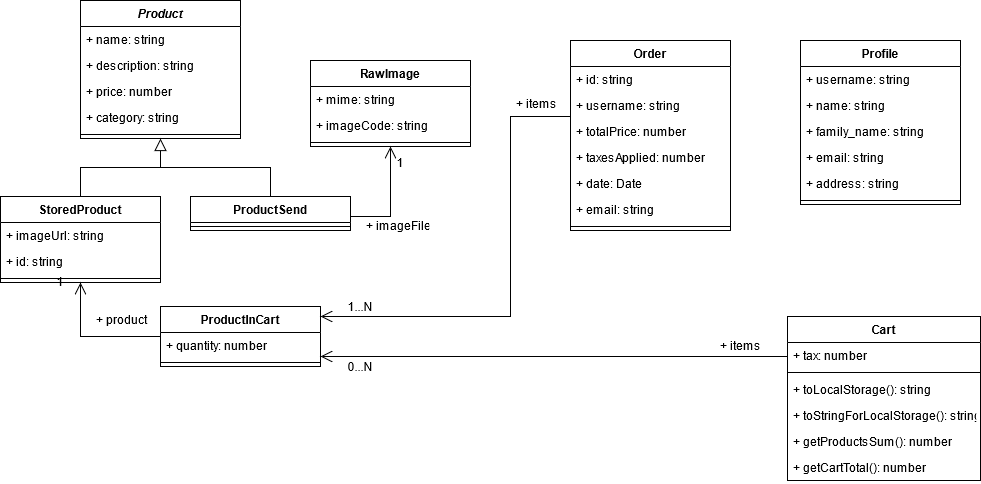
\includegraphics[scale=0.45]{res/Architettura/Frontend/img/class_frontend_types}\\
\caption{Diagramma delle classi dei tipi utilizzati per il modulo Front-end}
\end{figure}